%===============>> ГРУППА 8-1 МОДУЛЬ 3 <<=============
\setmodule{3}
%
%===============>>  Занятие 1  <<===============
%
\begin{class}[number=1]
\begin{listofex}
	\item Вычислить:
	\begin{enumcols}[itemcolumns=3]
		\item \exercise{1665}
		\item \exercise{1775}
		\item \exercise{1221}
		\item \exercise{1578}
		\item \exercise{1589}
		\item \exercise{1137}
		\item \exercise{2984}
	\end{enumcols}
	\item Некоторая компания продает свою продукцию по цене\(  p=500  \)руб. за единицу, переменные затраты на производство одной единицы продукции составляют  \( v=300 \) руб., постоянные расходы предприятия \( f=700000 \) руб. в месяц. Месячная операционная прибыль предприятия (в рублях) вычисляется по формуле  \( \pi(q)=q(p-v)-f \). Определите месячный объeм производства\(  q \) (единиц продукции), при котором месячная операционная прибыль предприятия будет равна \( 300000 \) руб.
	\item Зависимость объёма спроса \( q \) (единиц в месяц) на продукцию предприятия – монополиста от цены \( p \) (тыс. руб.) задаётся формулой \( q=100-10p \). Выручка предприятия за месяц \( r \) (в тыс. руб.) вычисляется по формуле \( r(p)=q\cdot p \). Определите наибольшую цену \( p \), при которой месячная выручка \( r(p) \) составит не менее \( 240 \) тыс. руб. Ответ приведите в тыс. руб.
	\item По закону Ома для полной цепи сила тока, измеряемая в амперах, равна \( I=\dfrac{\sigma}{R+r} \), где \(\sigma\) – ЭДС источника (в вольтах), \(r=2\) Ом – его внутреннее сопротивление, \(R\) – сопротивление цепи (в омах). При каком наименьшем сопротивлении цепи сила тока будет составлять не более \(40\% \) от силы тока короткого замыкания \( I_{кз} =\dfrac{\sigma}{r}\)? (Ответ выразите в омах).
	\item Гоночный автомобиль разгоняется на прямолинейном участке шоссе с постоянным ускорением \( a \) км/ч\( ^2 \). Скорость \( v \)  в конце пути вычисляется по формуле \( v=\sqrt{2la} \), где \( l \) – пройденный автомобилем путь в км. Определите ускорение, с которым должен двигаться автомобиль, чтобы, проехав \( 250 \) метров, приобрести скорость \( 60 \)км/ч. Ответ выразите в км/ч\( ^2 \).
	\item Расстояние (в км) от наблюдателя, находящегося на небольшой высоте \( h \) километров над землeй, до наблюдаемой им линии горизонта вычисляется по формуле \( l=\sqrt{2Rh} \), где \( R = 6400 \) (км) – радиус Земли. С какой высоты горизонт виден на расстоянии \(4\) километра? Ответ выразите в километрах.
	\item Фабрика выпускает сумки. В среднем на \( 110 \) качественных сумок приходится одиннадцать сумок со скрытыми дефектами. Найдите вероятность того, что купленная сумка окажется качественной. Результат округлите до сотых.
	\item На борту самолёта \( 13 \) мест рядом с запасными выходами и \( 19 \) мест за перегородками, разделяющими салоны. Остальные места неудобны для пассажира высокого роста. Пассажир В. высокого роста. Найдите вероятность того, что на регистрации при случайном выборе места пассажиру В. достанется удобное место, если всего в самолёте \( 200 \) мест.
	\item Девять одинаковых рубашек дешевле куртки на \( 10\% \). На сколько процентов четырнадцать таких же рубашек дороже куртки?
	\item Игорь и Паша красят забор за \( 15 \) часов. Паша и Володя красят этот же забор за \( 21 \) час, а Володя и Игорь – за \( 35 \) часов. За сколько часов мальчики покрасят забор, работая втроем?
\end{listofex}
\end{class}
%
%===============>>  Занятие 2  <<===============
%
%\begin{class}[number=2]
%
%===============>>  Домашняя работа 1  <<===============
%
\begin{homework}[number=1]
\cheadbf{Модуль 3 Домашняя работа 1}
\begin{listofex}
	\item Вычислить:
	\begin{enumcols}[itemcolumns=3]
		\item \exercise{1689}
		\item \exercise{1776}
		\item \( \sqrt{7}\cdot\sqrt[4]{7}\cdot\sqrt[8]{7} \)
		\item \exercise{569}
		\item \exercise{588}
		\item \exercise{2994}
		\item \( 14\cos(-135\degree)\cdot\sin(-45\degree) \)
	\end{enumcols}
	\item При температуре \( 0^{\circ}  \) рельс имеет длину \( l_0=12,5 \)м. При возрастании температуры происходит тепловое расширение рельса, и его длина, выраженная в метрах, меняется по закону \( l(t^{\circ})=l_0(1+\alpha\cdot t^{\circ}) \), где  \( \alpha=1,2\cdot 10^{-5}(^{\circ}C)^{-1} \) – коэффициент теплового расширения, \( t^{\circ} \) – температура (в градусах Цельсия). При какой температуре рельс удлинится на \( 6 \) мм? Ответ выразите в градусах Цельсия.
	\item Некоторая компания продаёт свою продукцию по цене \( p = 600 \) руб. за единицу, переменные затраты на производство одной единицы продукции составляют \( v = 300 \) руб., постоянные расходы предприятия \( f = 700 000 \) руб. в месяц. Месячная операционная прибыль предприятия (в рублях) вычисляется по формуле \(g(q)=q(p-v)-f\). Определите месячный объём производства \( q \) (единиц продукции), при котором месячная операционная прибыль предприятия будет равна \( 500 000 \) руб.
	\item По закону Ома для полной цепи сила тока, измеряемая в амперах, равна \( I=\dfrac{\sigma}{R+r} \), где \(\sigma\) – ЭДС источника (в вольтах), \(r=4\) Ом – его внутреннее сопротивление, \(R\) – сопротивление цепи (в омах). При каком наименьшем сопротивлении цепи сила тока будет составлять не более \( 60\% \) от силы тока короткого замыкания \( I_{кз} =\dfrac{\sigma}{r}\)? (Ответ выразите в омах).
	\item На экзамен вынесено \( 60 \) вопросов, Андрей не выучил \( 3 \) из них. Найдите вероятность того, что ему попадется выученный вопрос.
	\item У Вити в копилке лежит \( 12 \) рублёвых, \( 6 \) двухрублёвых, \( 4 \) пятирублёвых и \( 3 \) десятирублёвых монеты. Витя наугад достаёт из копилки одну монету. Найдите вероятность того, что оставшаяся в копилке сумма составит более \( 70 \) рублей.
	\item Игорь и Паша красят забор за \( 21 \) час. Паша и Володя красят этот же забор за \( 28 \) часов, а Володя и Игорь – за \( 60 \) часов. За сколько часов мальчики покрасят забор, работая втроем?
	\item Четыре одинаковые рубашки дешевле куртки на \( 8\% \). На сколько процентов пять таких же рубашек дороже куртки?
	\item Решить уравнение:
	\begin{enumcols}[itemcolumns=2]
		\item \( \sqrt{\dfrac{1}{15x-4}}=0,2 \)
		\item \( \log_5(x^2+2x)=\log_5(x^2+10) \)
		\item \( \left( \dfrac{1}{3} \right)^{x-8}=\dfrac{1}{9} \)
	\end{enumcols}
\end{listofex}
\end{homework}
%\newpage
%\title{Занятие №3}
%\begin{listofex}
%	
%\end{listofex}
%\newpage
%\title{Занятие №4}
%\begin{listofex}
%	
%\end{listofex}
%
%===============>>  Домашняя работа 2  <<===============
%
\begin{homework}[number=2]
\begin{listofex}
	\item В кармане у Пети было четыре конфеты — «Белочка», «Василёк», «Красная шапочка» и «Маска», а также ключи от квартиры. Вынимая ключи, Петя случайно выронил из кармана одну конфету. Найдите вероятность того, что потерялась конфета «Василёк».
	\item В сборнике билетов по математике всего 60 билетов, в 9 из них встречается вопрос по теме "Геометрия". Найдите вероятность того, что в случайно выбранном на экзамене билете школьнику достанется вопрос по теме "Геометрия".
	\item В ходе распада радиоактивного изотопа его масса уменьшается по закону \( m(t)=m_0\cdot2^{-t/T} \), где \( m_0 \) - начальная масса изотопа,  \( t \) - время, прошедшее от начального момента, \( T \) - период полураспада. В начальный момент времени масса изотопа \( 52 \) мг. Период его полураспада составляет \( 9  \) мин. Найдите, через сколько минут масса изотопа будет равна \( 13  \) мг.
	\item Расстояние от наблюдателя, находящегося на небольшой высоте  h километров над землёй, до наблюдаемой им линии горизонта вычисляется по формуле \( l=\sqrt{2Rh} \), где \( R=6400 \) км - радиус Земли. С какой высоты горизонт виден на расстоянии \( 32 \) километра? Ответ выразите в километрах.
	\item Теплоход проходит по течению реки до пункта назначения \( 200 \) км и после стоянки возвращается в пункт отправления. Найдите скорость течения, если скорость теплохода в неподвижной воде равна \( 15 \) км/ч, стоянка длится 10 часов, а в пункт отправления теплоход возвращается через \( 40 \) часов после отплытия из него. Ответ дайте в км/ч.
	\item \begin{minipage}[t]{0.67\textwidth}
		На рисунке изображен график функции \( f(x)=kx+b \). Найдите \( f(-9) \).
	\end{minipage}
	\begin{minipage}[c]{0.2\textwidth}
		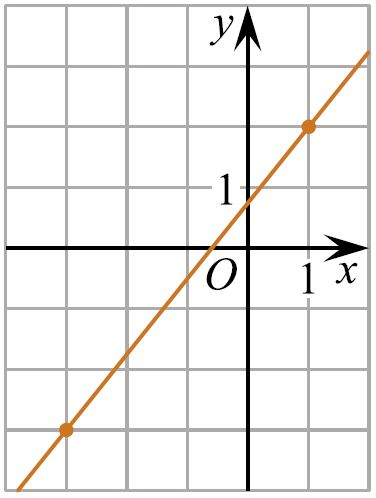
\includegraphics[align=t, width=0.8\textwidth]{pics/G112M3C2-1}
	\end{minipage}
	\item Найдите корень уравнения
	\( \sqrt{\dfrac{6}{4x-54}}=\dfrac{1}{7} \)
\end{listofex}
\end{homework}
%\newpage
%\title{Занятие №5}
%\begin{listofex}
%	
%\end{listofex}
%\newpage
%\title{Занятие №6}
%\begin{listofex}
%	
%\end{listofex}
%\newpage
%\title{Домашняя работа №3}
%\begin{listofex}
%	
%\end{listofex}
%\newpage
%\title{Подготовка к проверочной работе}
%\begin{listofex}
%	
%\end{listofex}
%\newpage
%\title{Проверочная работа}
%\title{Вариант 1}
%\begin{listofex}
%	
%\end{listofex}
%\newpage
%\title{Проверочная работа}
%\begin{listofex}
%	
%\end{listofex}